Part 2 uses ReducedMNIST, a reduced version of the MNIST dataset, with the following assignment-compliant split:

\begin{itemize}
    \item Original MNIST training set: 60,000 images total.
    \item Original MNIST test set: 10,000 images total.
    \item The script \texttt{part2\_reduced\_mnist.py} downloads MNIST and creates a reduced version of the dataset, called ReducedMNIST, with the following split:
        \begin{itemize}
            \item ReducedMNIST training set: 1000 images for each digit (10000 total).
            \item ReducedMNIST test set: 200 images for each digit (2000 total).
        \end{itemize}
\end{itemize}

\subsection{Feature Extraction}

Three feature extraction methods were used:

\begin{itemize}
    \item \textbf{DCT}: a $15 \times 15$ low-frequency block, giving 225 features.
    \item \textbf{PCA}: enough principal components to preserve at least 95\% of the total variance.
    \item \textbf{HOG}: histogram-of-oriented-gradients features extracted from each image.
\end{itemize}

\subsection{Classifiers}

Two classifier families were evaluated:

\begin{itemize}
    \item \textbf{K-means clustering per class} with $K = 1, 4, 16, 32$.
    \item \textbf{SVM} with a linear kernel and a nonlinear kernel.
\end{itemize}

For the nonlinear SVM result, the kernel used was \textbf{RBF} with \texttt{gamma = scale}.

\subsection{Results Summary}

Table~\ref{tab:part2_results} summarizes the final Part 2 results. Processing time is the total of feature extraction, training, and testing.

\begin{table}[H]
\centering
\caption{Part 2 comparison of features and classifiers}
\label{tab:part2_results}
\resizebox{\textwidth}{!}{
\begin{tabular}{llcccccc}
\toprule
\multicolumn{2}{c}{\textbf{}} & \multicolumn{2}{c}{\textbf{DCT}} & \multicolumn{2}{c}{\textbf{PCA}} & \multicolumn{2}{c}{\textbf{HOG}} \\
\cmidrule(lr){3-4} \cmidrule(lr){5-6} \cmidrule(lr){7-8}
\textbf{Classifier} & \textbf{Setting} & \textbf{Accuracy} & \textbf{Processing Time} & \textbf{Accuracy} & \textbf{Processing Time} & \textbf{Accuracy} & \textbf{Processing Time} \\
\midrule
K-means Clustering & 1  & 78.10\% & 1.8831 s & 85.20\% & 0.8123 s & 89.50\% & 5.4810 s \\
K-means Clustering & 4  & 84.40\% & 1.0484 s & 82.60\% & 1.1766 s & 92.00\% & 7.3776 s \\
K-means Clustering & 16 & 88.75\% & 2.2338 s & 85.70\% & 2.1196 s & 94.35\% & 13.5238 s \\
K-means Clustering & 32 & 89.65\% & 3.8399 s & 85.60\% & 3.5880 s & 93.95\% & 21.7835 s \\
SVM & Linear      & 90.25\% & 2.3988 s & 90.65\% & 3.1937 s & 97.45\% & 11.2708 s \\
SVM & Nonlinear*  & 95.55\% & 4.2029 s & 95.15\% & 5.5291 s & 97.15\% & 24.9506 s \\
\bottomrule
\end{tabular}
}
\end{table}

\noindent * Nonlinear kernel = RBF, \texttt{gamma = scale}.

\subsection{Best Results and Confusion Matrices}

The best K-means result was \textbf{K-means with $K=16$ using HOG}, with an accuracy of \textbf{94.35\%}. The best SVM result was \textbf{linear SVM using HOG}, with an accuracy of \textbf{97.45\%}. As required by the assignment, only the best result from each classifier family is shown as a confusion matrix.

\begin{figure}[H]
\centering
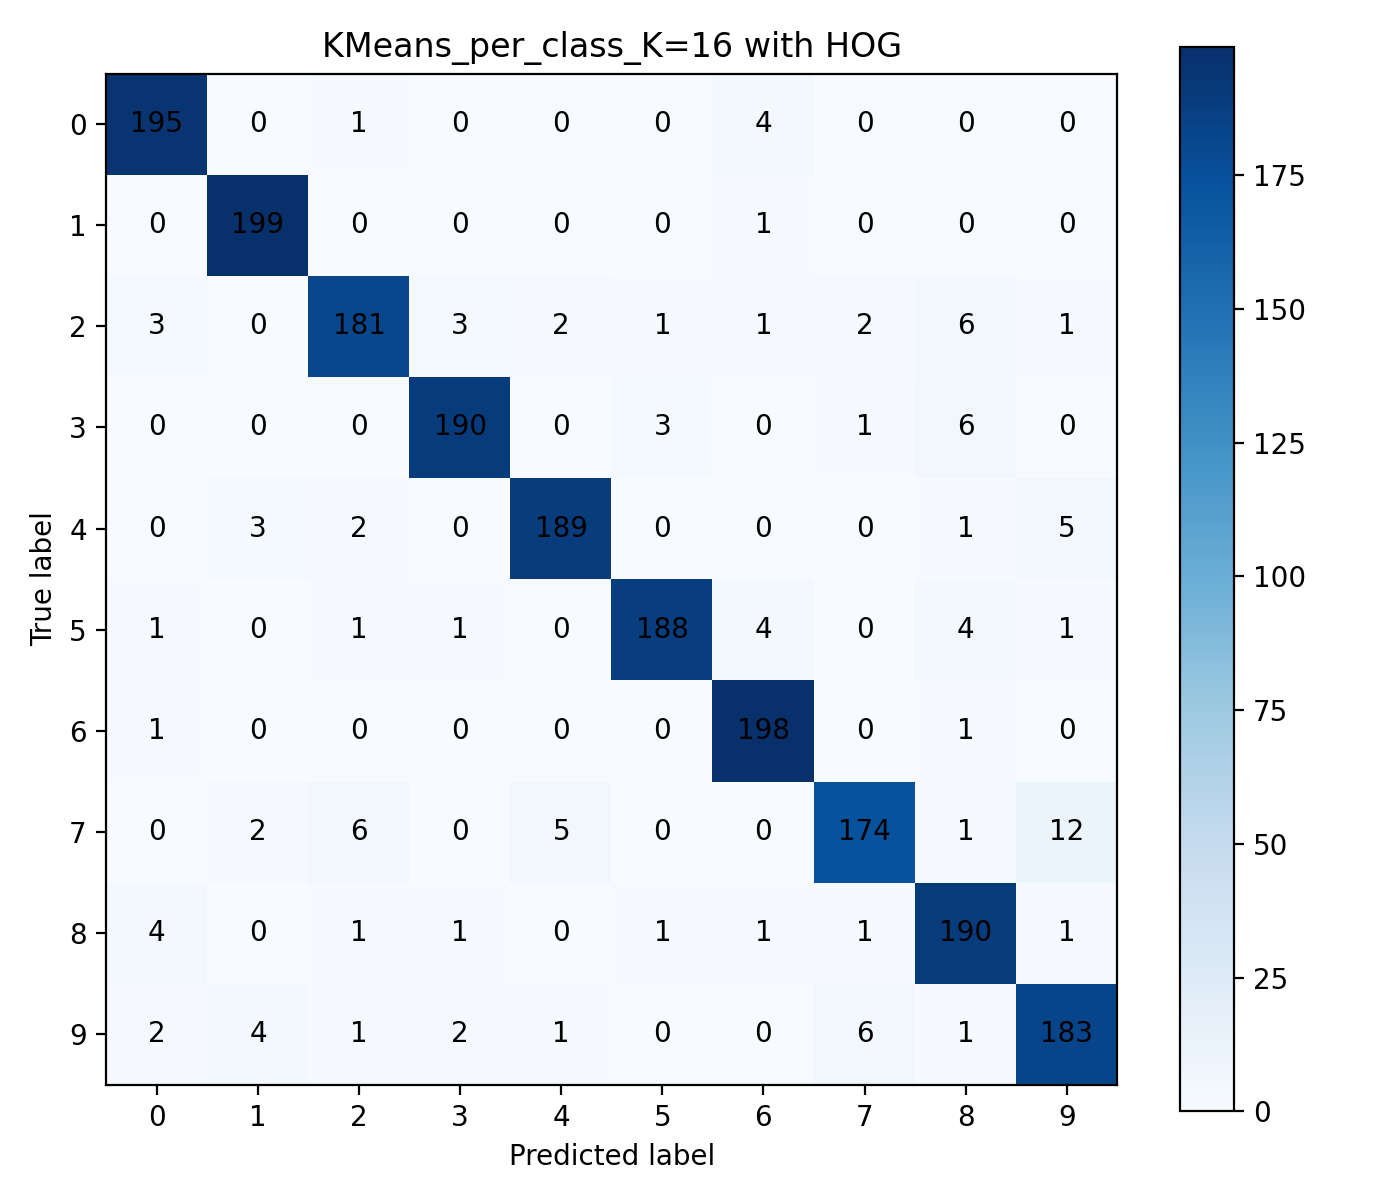
\includegraphics[width=0.68\textwidth]{figures/KMeans_per_class_K=16_HOG_confusion.png}
\caption{Confusion matrix for the best K-means result: K-means ($K=16$) with HOG features.}
\end{figure}

\begin{figure}[H]
\centering
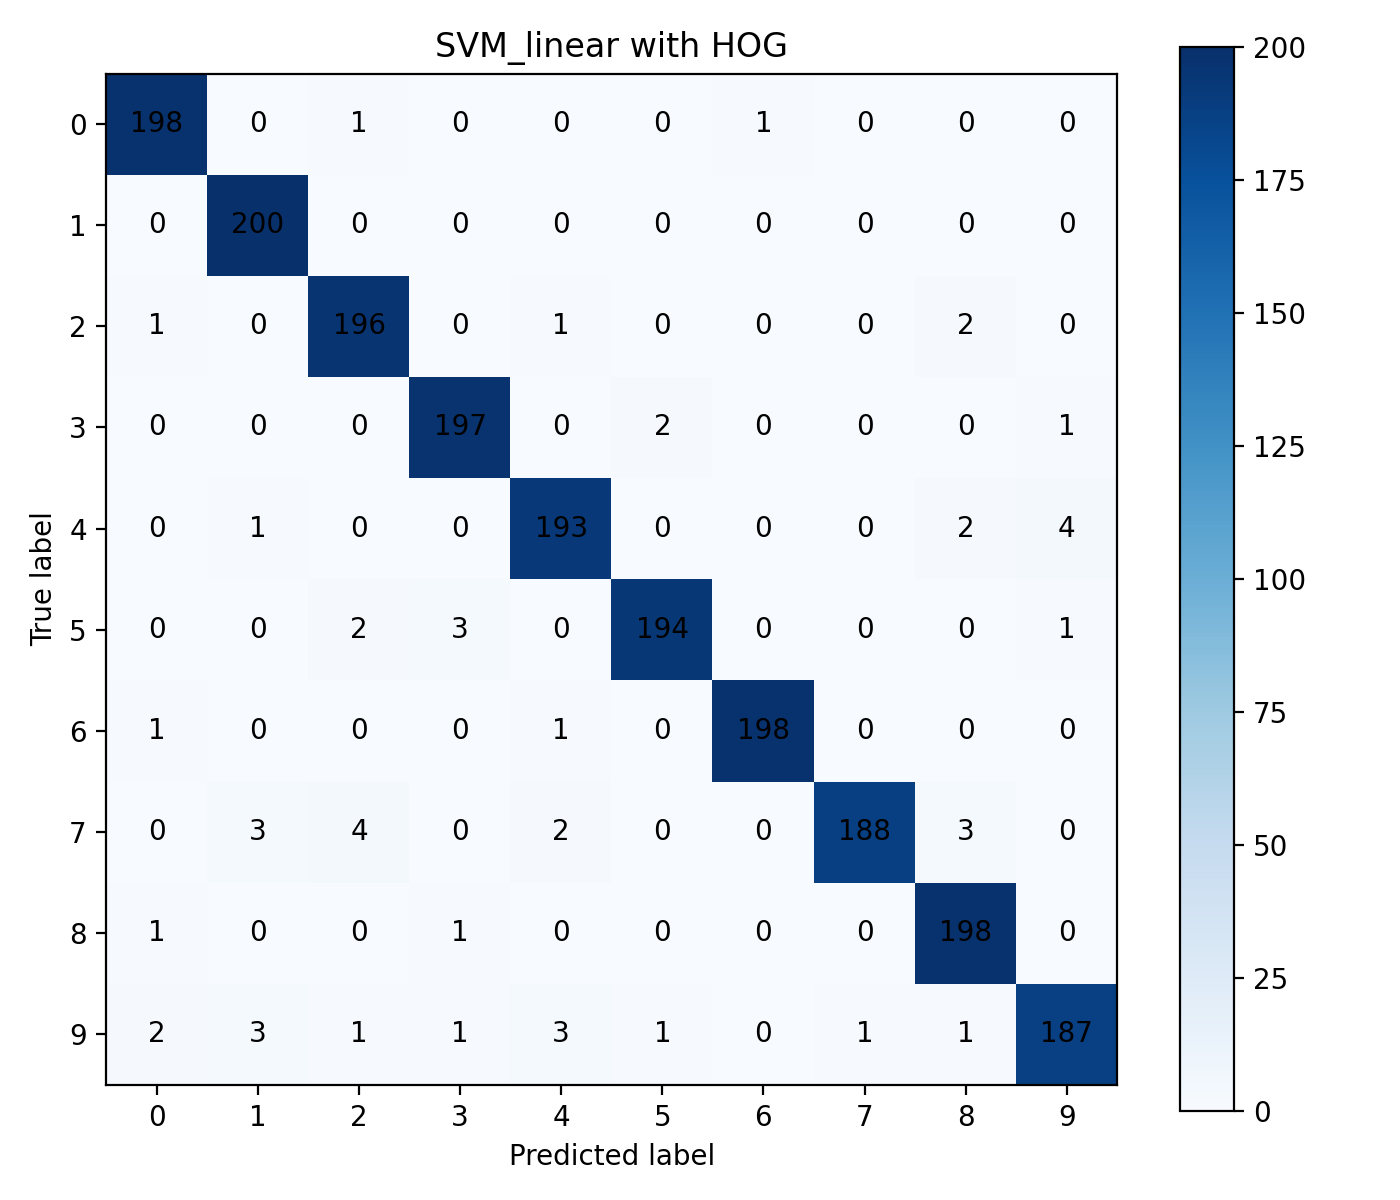
\includegraphics[width=0.68\textwidth]{figures/SVM_linear_HOG_confusion.png}
\caption{Confusion matrix for the best SVM result: linear SVM with HOG features.}
\end{figure}

\subsection{Observations}

The results show that HOG features produced the strongest classification accuracy across both classifier families. The best overall result was obtained by \textbf{linear SVM with HOG}, reaching \textbf{97.45\%}. The best K-means result, \textbf{K=16 with HOG}, reached \textbf{94.35\%}, so the best SVM result was \textbf{3.10 percentage points} higher.

For DCT and PCA, the nonlinear SVM result was slightly better than the linear SVM result. For HOG, however, the linear SVM result was the strongest overall result in the full comparison table. In terms of speed, the fastest overall experiment was \textbf{K-means with $K=1$ using PCA}, with a total processing time of \textbf{0.8123 s}, but with lower accuracy than the best SVM and HOG-based results.

\subsection{Part 2 Conclusion}

Based on the current experiments, \textbf{HOG features combined with linear SVM} gave the best overall performance for the ReducedMNIST classification task. HOG consistently captured the digit structure better than DCT and PCA in the final results, while linear SVM achieved the highest measured test accuracy with a reasonable processing time.